% % Requires \usepackage{tikz}. Include inside a figure environment.
% % Illustrative alternatives for the same validated request.
% \begingroup
% \begin{tikzpicture}[x=1cm,y=1cm,>=stealth]
% \definecolor{outcometext}{HTML}{1E293B}
% \definecolor{outcomeline}{HTML}{475569}
% \definecolor{outcomeneutral}{HTML}{F8FAFC}
% \definecolor{outcomeapprove}{HTML}{26864A}
% \definecolor{outcomeapprovefill}{HTML}{E1F4E5}
% \definecolor{outcomereject}{HTML}{A43A3A}
% \definecolor{outcomerejectfill}{HTML}{FBE8E8}
% \definecolor{outcomefailure}{HTML}{B86F00}
% \definecolor{outcomefailurefill}{HTML}{FEEDCD}

% \tikzset{
%   outcomeExampleBox/.style={draw=outcomeline,fill=outcomeneutral,
%     rounded corners=2pt,line width=0.65pt,align=center,text=outcometext,
%     inner sep=3pt,outer sep=0pt,font=\sffamily\fontsize{8.5}{10.5}\selectfont},
%   outcomeExampleText/.style={align=center,text=outcometext,inner sep=0pt,
%     font=\sffamily\fontsize{8.5}{10.5}\selectfont},
%   outcomeExampleArrow/.style={->,draw=outcomeline,line width=0.75pt}
% }

% \path[use as bounding box] (-0.05,0.60) rectangle (14.35,7.65);

% % A common request makes the difference in evidence explicit.
% \node[outcomeExampleBox,text width=13.15cm,minimum height=1.0cm]
%   (exampleRequest) at (7.15,7.08)
%   {\textbf{Validated request: swap 50 USDT for WETH}\\
%    Specified protocol deployment and blockchain network};

% \node[outcomeExampleText,font=\sffamily\fontsize{8}{9.5}\selectfont]
%   at (7.15,6.26)
%   {Three illustrative evidence conditions for the same request};

% % Equal panels and evidence boxes.
% \draw[draw=outcomeline,rounded corners=3pt,line width=0.6pt]
%   (0,0.72) rectangle (4.40,5.95);
% \draw[draw=outcomeline,rounded corners=3pt,line width=0.6pt]
%   (4.95,0.72) rectangle (9.35,5.95);
% \draw[draw=outcomeline,rounded corners=3pt,line width=0.6pt]
%   (9.90,0.72) rectangle (14.30,5.95);

% \node[outcomeExampleText,font=\sffamily\bfseries\fontsize{9}{11}\selectfont]
%   at (2.20,5.57) {Relationships established};
% \node[outcomeExampleText,font=\sffamily\bfseries\fontsize{9}{11}\selectfont]
%   at (7.15,5.57) {Unsupported action};
% \node[outcomeExampleText,font=\sffamily\bfseries\fontsize{9}{11}\selectfont]
%   at (12.10,5.57) {Insufficient valid evidence};

% \node[outcomeExampleBox,text width=3.65cm,minimum height=1.80cm]
%   (approveEvidence) at (2.20,4.30)
%   {Sufficient, current, valid\\
%    evidence establishes all\\
%    mandatory execution\\
%    relationships.};
% \node[outcomeExampleBox,text width=3.65cm,minimum height=1.80cm]
%   (rejectEvidence) at (7.15,4.30)
%   {Knowledge is complete\\
%    and current. Valid evidence\\
%    establishes that the swap\\
%    is unsupported.};
% \node[outcomeExampleBox,text width=3.65cm,minimum height=1.80cm]
%   (failureEvidence) at (12.10,4.30)
%   {Required deployment\\
%    evidence is stale or\\
%    unavailable; action support\\
%    cannot be established.};

% % Outcome boxes have identical dimensions.
% \node[outcomeExampleBox,text width=3.65cm,minimum height=1.05cm,
%   draw=outcomeapprove,fill=outcomeapprovefill,
%   font=\sffamily\bfseries\fontsize{9}{11}\selectfont]
%   (approveOutcome) at (2.20,2.53) {APPROVE};
% \node[outcomeExampleBox,text width=3.65cm,minimum height=1.05cm,
%   draw=outcomereject,fill=outcomerejectfill,
%   font=\sffamily\bfseries\fontsize{9}{11}\selectfont]
%   (rejectOutcome) at (7.15,2.53) {REJECT};
% \node[outcomeExampleBox,text width=3.65cm,minimum height=1.05cm,
%   draw=outcomefailure,fill=outcomefailurefill,
%   font=\sffamily\bfseries\fontsize{9}{11}\selectfont]
%   (failureOutcome) at (12.10,2.53) {VERIFICATION\\FAILURE};

% \draw[outcomeExampleArrow] (approveEvidence.south) -- (approveOutcome.north);
% \draw[outcomeExampleArrow] (rejectEvidence.south) -- (rejectOutcome.north);
% \draw[outcomeExampleArrow] (failureEvidence.south) -- (failureOutcome.north);

% \node[outcomeExampleText,text width=3.80cm] at (2.20,1.43)
%   {Forward approved result\\to controlled execution checks};
% \node[outcomeExampleText,text width=3.80cm] at (7.15,1.43)
%   {Block execution;\\report the unsupported action};
% \node[outcomeExampleText,text width=3.80cm] at (12.10,1.43)
%   {Block execution;\\report insufficient valid evidence};
% \end{tikzpicture}
% \endgroup
\begingroup
\definecolor{vInk}{HTML}{24394F}
\definecolor{vLine}{HTML}{506479}
\definecolor{vNode}{HTML}{F3F6FA}
\definecolor{vOk}{HTML}{206642}
\definecolor{vOkBg}{HTML}{E4F2E9}
\definecolor{vNo}{HTML}{923537}
\definecolor{vNoBg}{HTML}{F8E9E7}
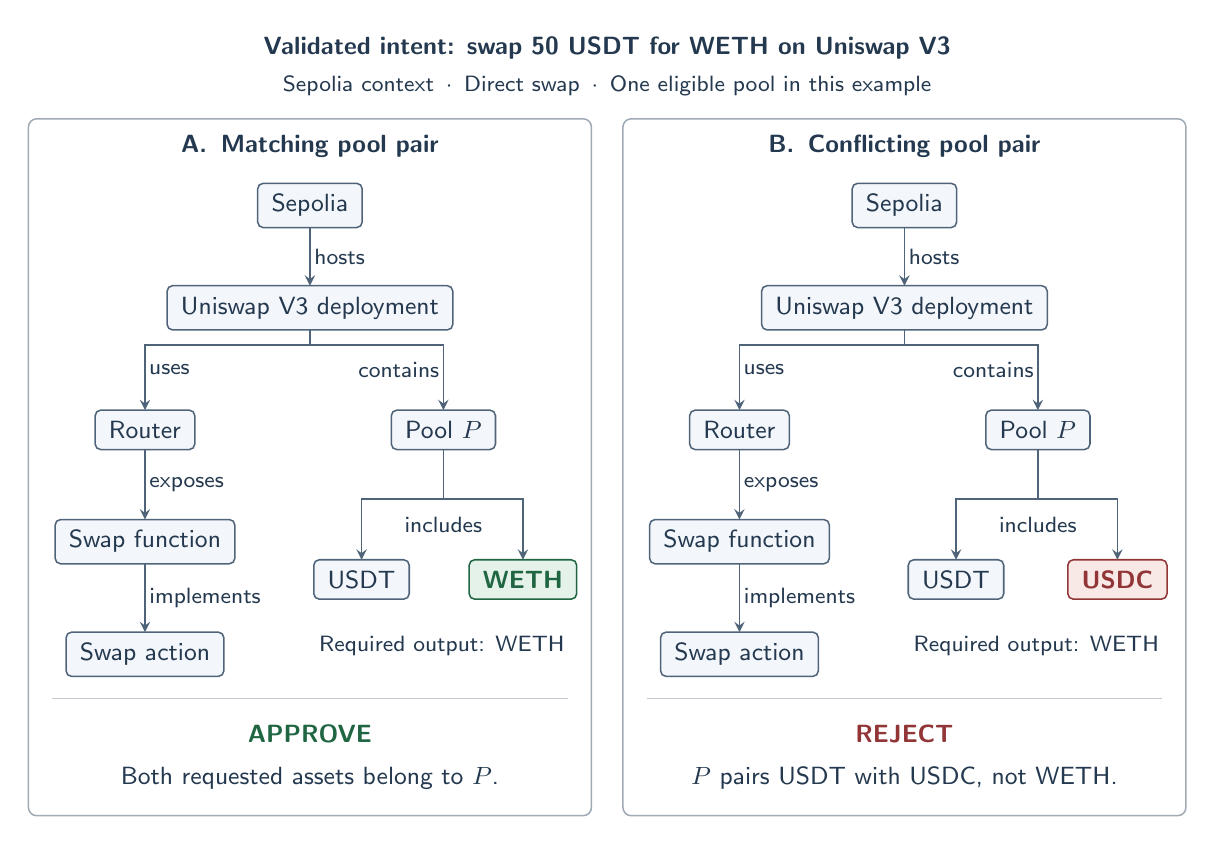
\begin{tikzpicture}[x=1cm,y=1cm,>=stealth,
  every node/.style={font=\sffamily\small,text=vInk,align=center},
  vertex/.style={draw=vLine,fill=vNode,rounded corners=2pt,
    line width=.55pt,inner xsep=5pt,inner ysep=4pt,outer sep=0pt},
  edge/.style={->,draw=vLine,line width=.65pt},
  verb/.style={font=\sffamily\footnotesize,inner sep=1.3pt},
  title/.style={font=\sffamily\bfseries\small}]
\node[title] at (7.35,9.75) {Validated intent: swap 50 USDT for WETH on Uniswap V3};
\node[font=\sffamily\footnotesize] at (7.35,9.27)
  {Sepolia context\enspace$\cdot$\enspace Direct swap\enspace$\cdot$\enspace One eligible pool in this example};
\foreach \dx/\lettertag/\heading/\otherasset/\decision/\ink/\tint in {
  0/A/Matching pool pair/WETH/APPROVE/vOk/vOkBg,
  7.55/B/Conflicting pool pair/USDC/REJECT/vNo/vNoBg}{
  \begin{scope}[xshift=\dx cm]
    \draw[draw=vLine!55,rounded corners=3pt,line width=.55pt]
      (0,0) rectangle (7.15,8.85);
    \node[title] at (3.575,8.50) {\lettertag.\enspace \heading};
    \node[vertex] (net) at (3.575,7.75) {Sepolia};
    \node[vertex] (dep) at (3.575,6.45) {Uniswap V3 deployment};
    \node[vertex] (router) at (1.48,4.90) {Router};
    \node[vertex] (pool) at (5.27,4.90) {Pool $P$};
    \node[vertex] (func) at (1.48,3.48) {Swap function};
    \node[vertex] (action) at (1.48,2.05) {Swap action};
    \node[vertex] (assetA) at (4.23,3.00) {USDT};
    \node[vertex,draw=\ink,fill=\tint,text=\ink,font=\sffamily\bfseries\small]
      (assetB) at (6.28,3.00) {\otherasset};
    \draw[edge] (net.south) -- node[verb,right] {hosts} (dep.north);
    \draw[edge] (dep.south) -- (3.575,5.98) -| (router.north);
    \draw[edge] (dep.south) -- (3.575,5.98) -| (pool.north);
    \node[verb,right] at (1.48,5.66) {uses};
    \node[verb,left] at (5.27,5.66) {contains};
    \draw[edge] (router.south) -- node[verb,right] {exposes} (func.north);
    \draw[edge] (func.south) -- node[verb,right] {implements} (action.north);
    \draw[edge] (pool.south) -- (5.27,4.02) -- (4.23,4.02) -- (assetA.north);
    \draw[edge] (pool.south) -- (5.27,4.02) -- (6.28,4.02) -- (assetB.north);
    \node[verb] at (5.27,3.70) {includes};
    \node[font=\sffamily\footnotesize] at (5.25,2.15) {Required output: WETH};
    \draw[draw=vLine!35] (.30,1.49) -- (6.85,1.49);
    \node[title,text=\ink] at (3.575,1.04) {\decision};
    \def\firstpanel{A}
    \ifx\lettertag\firstpanel
      \node at (3.575,.48) {Both requested assets belong to $P$.};
    \else
      \node at (3.575,.48) {$P$ pairs USDT with USDC, not WETH.};
    \fi
  \end{scope}}
\end{tikzpicture}
\endgroup